% slides_sim_fakegeo_en.tex -- cardiac-sim-fakegeo presentation (English)
% Compile:  pdflatex slides_sim_fakegeo_en.tex   (or xelatex)
%           fig_mesh.png in the same directory is embedded automatically.
\documentclass[aspectratio=169,11pt]{beamer}
\usetheme{Madrid}
\usecolortheme{whale}
\usepackage{booktabs}
\usepackage{array}
\usepackage{multirow}
\usepackage{amsmath}
\usepackage{xcolor}
\usepackage{graphicx}
\definecolor{good}{RGB}{22,140,74}
\definecolor{bad}{RGB}{200,38,38}
\definecolor{hl}{RGB}{234,88,12}
\newcommand{\up}{\textcolor{bad}{$\uparrow$}}
\newcommand{\dn}{\textcolor{good}{$\downarrow$}}
\setbeamertemplate{navigation symbols}{}
\setbeamerfont{footline}{size=\tiny}

\title[cardiac-sim-fakegeo]{Coupled Forward ECG on Real-Geometry FEM:\\ASM vs.\ sASM Domain-Decomposition Preconditioning}
\subtitle{Branch \texttt{cardiac-sim-fakegeo} $\cdot$ algorithm study (numerical linear algebra / domain decomposition)}
\author{tianhaoma-hpc}
\date{MFEM 4.9 + PETSc 3.19 $\cdot$ all numbers measured on \texttt{heart.msh}}

\begin{document}

\begin{frame}\titlepage\end{frame}

\begin{frame}{Overview: nature of the study and the main thread}
\textbf{Nature}: a Krylov-preconditioning / domain-decomposition (Additive Schwarz) \emph{algorithm} study. The vehicle is a coupled-PDE forward problem, but the \emph{object of study is how the linear systems converge faster and scale}.
\vspace{0.6em}
\begin{block}{Pipeline}
\[
\underbrace{\text{Sys1 } V_m}_{\text{parabolic}\cdot\text{local}}\ \xrightarrow{V_m(t)}\
\underbrace{\text{Sys2 } u_e}_{\text{singular elliptic}\cdot\text{global}}\ \xrightarrow{\text{Dirichlet}}\
\underbrace{\text{Sys3 } \varphi}_{\text{elliptic}\cdot\text{nonsingular}}\ \to\ \text{ECG}
\]
\end{block}
\textbf{This deck focuses on}: the problem definition, the mesh, and the \textbf{ASM(BASIC)} vs.\ \textbf{sASM(scaled/restricted)} \textbf{iteration counts} and \textbf{wall-clock time} on the three systems.
\end{frame}

\begin{frame}{Problem: algebraic characterization of the three systems}
Each time step solves three SPD (semi-)definite systems (\texttt{heart.msh}, Sys2 has $10085$ unknowns):
\vspace{0.4em}
\begin{table}\small
\begin{tabular}{@{}lllc@{}}
\toprule
System & Equation & Algebraic type & baseline iters \\
\midrule
\textbf{Sys1} $V_m$ & $\left(\tfrac1{\Delta t}M+\tfrac12K\right)V_m=b$ & parabolic / \textbf{mass-dominated} / nonsingular & CG+ICC $\sim$13 \\
\textbf{Sys2} $u_e$ & $K_{\sigma_i+\sigma_e}\,u_e=-K_{\sigma_i}V_m$ & elliptic / \textbf{pure-Neumann singular} / global & $\sim$82--96 \\
\textbf{Sys3} $\varphi$ & $K_{\sigma_o}\varphi=0$, interface Dirichlet & elliptic / nonsingular / global & $\sim$62--66 \\
\bottomrule
\end{tabular}
\end{table}
\vspace{0.3em}
\textbf{Sys2 is the only hard one} (singular $+$ elliptic $+$ global):
\begin{itemize}
\item $K\mathbf{1}=0$: null space $=$ constants $=$ one slow global mode $\Rightarrow$ de-mean the RHS $+$ \texttt{MatSetNullSpace} (project the constant mode out every CG iteration).
\item global elliptic $\Rightarrow$ a one-level domain decomposition propagates only one subdomain hop per iteration; more subdomains $=$ slower (the core theme below).
\end{itemize}
\end{frame}

\begin{frame}{Geometry: conforming heart-in-torso domains}
\centerline{\IfFileExists{fig_geom.png}{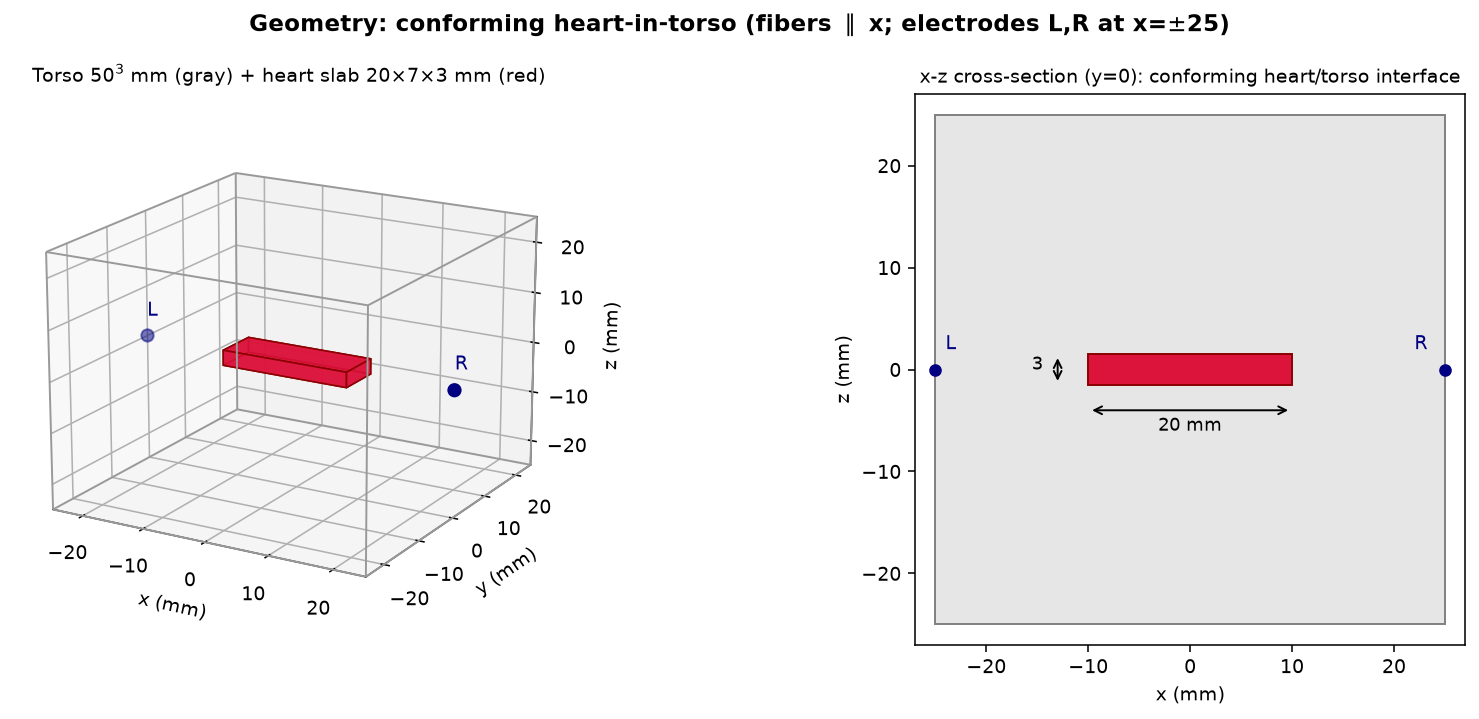
\includegraphics[width=0.82\linewidth]{fig_geom.png}}%
{\fbox{\parbox{0.7\linewidth}{\centering \texttt{fig\_geom.png} --- run \texttt{python3 plot\_geom\_mesh.py}}}}}
\vspace{0.3em}
{\footnotesize Heart slab $20\times7\times3$ mm centered in a $50^3$ mm torso; \textbf{conforming} interface (Gmsh \texttt{BooleanFragments} $\Rightarrow$ shared interface surface). Anisotropic $\sigma$, fibers $\parallel x$; electrodes L,R at $x=\pm25$; subdomains $=$ MPI ranks (METIS).\par}
\end{frame}

\begin{frame}{Mesh: unstructured P1 tetrahedra (real connectivity)}
\centerline{\IfFileExists{fig_meshview.png}{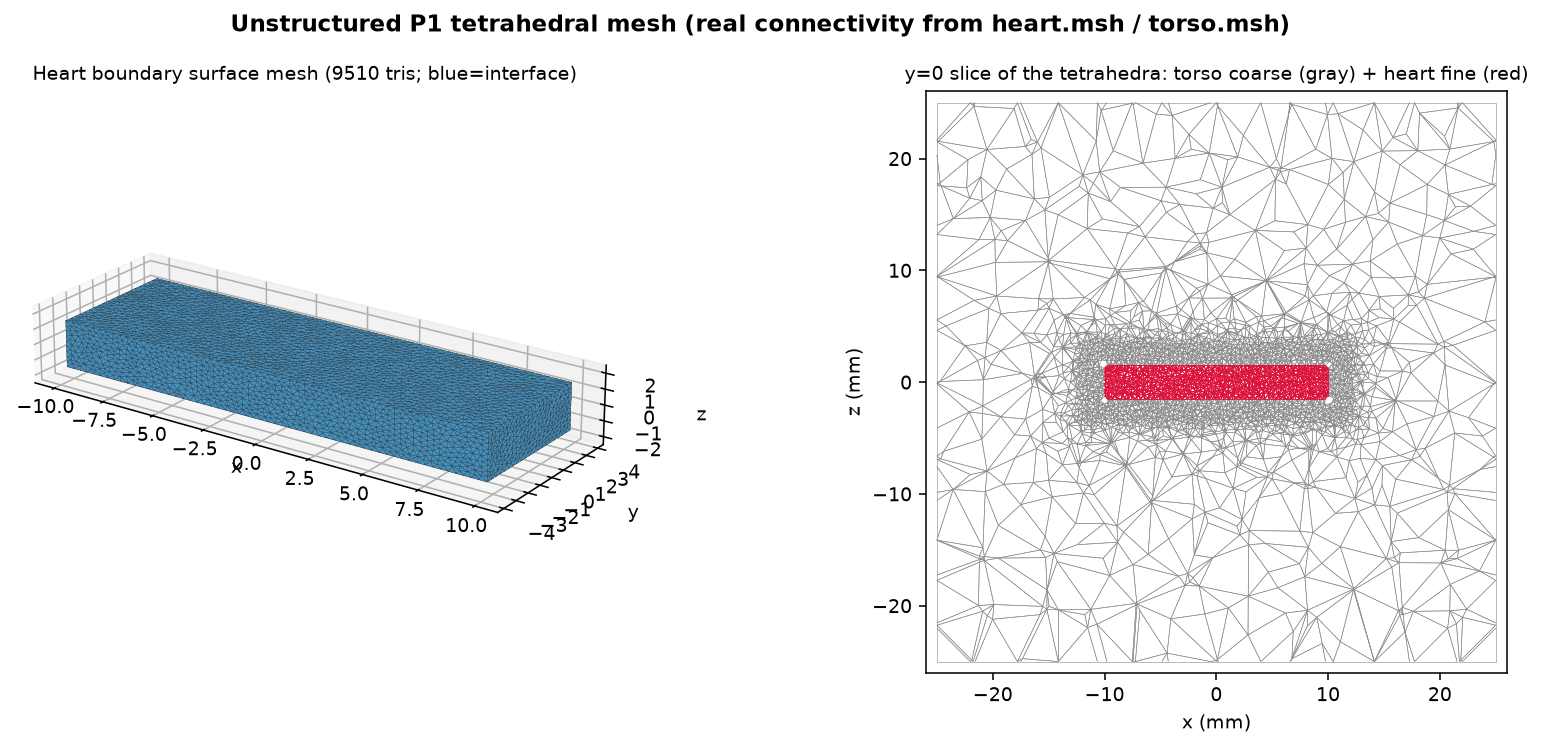
\includegraphics[width=0.80\linewidth]{fig_meshview.png}}%
{\fbox{\parbox{0.7\linewidth}{\centering \texttt{fig\_meshview.png} --- run \texttt{python3 plot\_geom\_mesh.py}}}}}
\vspace{0.3em}
\centerline{\scriptsize
\begin{tabular}{@{}lrrr@{\hskip 1.5em}l@{}}
heart & $10\,085$ nodes & $47\,582$ tets & $9\,510$ tris & \multirow{2}{*}{interface shared dofs: $4\,757$;\ \ $y{=}0$ slice: heart $\sim$0.5 mm, torso $\sim$3 mm} \\
torso & $36\,229$ nodes & $206\,647$ tets & $12\,112$ tris & \\
\end{tabular}}
\end{frame}

\begin{frame}{Method: ASM(BASIC) vs.\ sASM(scaled / restricted)}
One-level additive Schwarz, blocks $=$ METIS subdomains, sub-solve $=$ ICC(0):
\[
M_{\text{ASM}}^{-1}=\sum_{i} R_i^\top A_i^{-1} R_i,\qquad
A_i=R_i A R_i^\top\ (\text{overlap } O\text{ layers})
\]
\begin{block}{The key difference --- overlap \emph{multiplicity} (over-count)}
\begin{itemize}
\item \textbf{ASM(BASIC)}: overlap dofs get \emph{one contribution from each} overlapping subdomain $\Rightarrow$ \textbf{over-counting} in the overlap, which corrupts the operator spectrum and can even \emph{increase iterations with overlap}.
\item \textbf{sASM}: a diagonal partition of unity $D^{-1/2}(\cdot)D^{-1/2}$ cancels the over-count ($D=$ multiplicity) $\Rightarrow$ overlap works \emph{as intended}, iterations drop with overlap.
\end{itemize}
\end{block}
\[
M_{\text{sASM}}^{-1}=D^{-1/2}\Big(\textstyle\sum_i R_i^\top A_i^{-1} R_i\Big)D^{-1/2}
\]
At $O{=}0$ (no overlap) there is no over-count, so \textbf{ASM $\equiv$ sASM}.
\end{frame}

\begin{frame}{Iterations: ASM vs.\ sASM ($n_p{=}4$, rtol $10^{-8}$, ICC(0))}
\begin{table}\small
\begin{tabular}{@{}llccl@{}}
\toprule
System & $O$ & ASM(BASIC) & sASM & note \\
\midrule
\multirow{3}{*}{Sys1 $V_m$}
 & 0 & 11 & 11 & $O{=}0$: equal \\
 & 1 & 13 \up & \textbf{8} \dn & \\
 & 2 & 13 \up & \textbf{8} \dn & \\
\midrule
\multirow{3}{*}{Sys2 $u_e$ (singular)}
 & 0 & 82 & 82 & \\
 & 1 & 92 \up & \textbf{74} \dn & \\
 & 2 & 93 \up & \textbf{74} \dn & \\
\midrule
\multirow{3}{*}{Sys3 $\varphi$}
 & 0 & 62 & 62 & \\
 & 1 & 88 \up & \textbf{53} \dn & \\
 & 2 & 94 \up & \textbf{53} \dn & \\
\bottomrule
\end{tabular}
\end{table}
\vspace{-0.3em}
\footnotesize \textcolor{bad}{$\uparrow$ ASM iterations \emph{rise} with overlap} (over-count); \textcolor{good}{$\downarrow$ sASM \emph{falls}} with overlap (overlap works correctly).
\end{frame}

\begin{frame}{Iterations: ASM vs.\ sASM ($n_p{=}8$, more subdomains $\Rightarrow$ stronger anomaly)}
\begin{table}\small
\begin{tabular}{@{}llccl@{}}
\toprule
System & $O$ & ASM(BASIC) & sASM & note \\
\midrule
\multirow{3}{*}{Sys1 $V_m$}
 & 0 & 13 & 13 & \\
 & 1 & 18 \up & \textbf{8} \dn & \\
 & 2 & 19 \up & \textbf{8} \dn & \\
\midrule
\multirow{3}{*}{Sys2 $u_e$ (singular)}
 & 0 & 79 & 79 & \\
 & 1 & 117 \up & \textbf{73} \dn & \\
 & 2 & 123 \up & \textbf{71} \dn & \\
\midrule
\multirow{3}{*}{Sys3 $\varphi$}
 & 0 & 66 & 66 & \\
 & 1 & 93 \up & \textbf{55} \dn & \\
 & 2 & 109 \up & \textbf{53} \dn & \\
\bottomrule
\end{tabular}
\end{table}
\vspace{-0.3em}
\footnotesize Most extreme: Sys3 ASM $O{:}0{\to}2$ \textcolor{bad}{$66{\to}93{\to}109$ ($+65\%$)}; sASM \textcolor{good}{$66{\to}55{\to}53$ ($-20\%$)}.
\end{frame}

\begin{frame}{Wall-clock: ASM vs.\ sASM (ms; KSP+PCASM setup $+$ solve, avg of $20$)}
\begin{columns}[T]
\begin{column}{0.5\textwidth}
\centering $n_p=4$\\[0.2em]
\begin{table}\scriptsize
\begin{tabular}{@{}llrr@{}}
\toprule
System & $O$ & ASM & sASM \\
\midrule
\multirow{3}{*}{Sys1}&0&3.66&3.79\\&1&5.27&\textbf{5.60}\\&2&6.88&\textbf{5.22}\dn\\
\midrule
\multirow{3}{*}{Sys2}&0&15.39&18.85\\&1&21.50&\textbf{17.60}\dn\\&2&24.33&\textbf{19.39}\dn\\
\midrule
\multirow{3}{*}{Sys3}&0&43.59&46.99\\&1&68.10&\textbf{44.36}\dn\\&2&80.18&\textbf{52.57}\dn\\
\bottomrule
\end{tabular}
\end{table}
\end{column}
\begin{column}{0.5\textwidth}
\centering $n_p=8$\\[0.2em]
\begin{table}\scriptsize
\begin{tabular}{@{}llrr@{}}
\toprule
System & $O$ & ASM & sASM \\
\midrule
\multirow{3}{*}{Sys1}&0&5.37&5.62\\&1&8.93&\textbf{7.89}\dn\\&2&14.90&\textbf{8.91}\dn\\
\midrule
\multirow{3}{*}{Sys2}&0&24.48&26.73\\&1&45.72&\textbf{28.94}\dn\\&2&53.15&\textbf{32.83}\dn\\
\midrule
\multirow{3}{*}{Sys3}&0&72.98&59.58\dn\\&1&96.81&\textbf{71.03}\dn\\&2&133.24&\textbf{77.17}\dn\\
\bottomrule
\end{tabular}
\end{table}
\end{column}
\end{columns}
\vspace{0.2em}
\footnotesize For $O{\ge}1$, sASM is \textbf{both fewer iterations and faster wall-clock}; for ASM, overlap \emph{costs time and raises iterations}. $n_p{=}8$ Sys3 $O{=}2$: ASM $109$it$/133$ms vs.\ sASM $53$it$/77$ms ($\sim1.7\times$).
\end{frame}

\begin{frame}{Key finding: the overlap anomaly}
\begin{block}{Observation}
Adding overlap to one-level \textbf{ASM(BASIC)} \emph{raises} iterations and slows wall-clock; adding overlap to \textbf{sASM} \emph{lowers both}.
\end{block}
\begin{block}{Mechanism: overlap anomaly $=$ over-count $\times$ inexactness}
\begin{itemize}
\item overlap dofs counted once per subdomain $\Rightarrow$ BASIC \textbf{amplifies} in the overlap ($\|M^{-1}\|$ too large), degrading the spectrum.
\item ICC(0) sub-solves are \emph{inexact}, so the amplified error is not absorbed by an exact local solve $\Rightarrow$ iterations climb.
\item the $D^{-1/2}$ partition of unity in sASM cancels the over-count exactly $\Rightarrow$ restores the correct behavior ``more overlap $=$ faster information transport''.
\end{itemize}
\end{block}
\textbf{Conclusion}: on real-geometry FEM, \textbf{scaled/restricted ASM is the correct way to use overlapping DD}; BASIC overlap is harmful here. More subdomains ($n_p{:}4{\to}8$) $\Rightarrow$ stronger anomaly, underscoring that \emph{scalability} needs the correct weighting (and, later, a coarse space).
\end{frame}

\begin{frame}{Summary and outlook}
\begin{itemize}
\item \textbf{Problem}: coupled forward ECG on three systems; Sys2 (singular pure-Neumann elliptic) is the only hard one and the target of the preconditioning study.
\item \textbf{Mesh}: conforming unstructured tet P1-FEM, heart $10085$ dof / $47582$ tets, torso $36229$ / $206647$.
\item \textbf{ASM vs.\ sASM} (measured, $n_p{=}4,8$):
  \begin{itemize}
  \item ASM(BASIC) iterations \textcolor{bad}{rise with overlap} (over-count), wall-clock slower;
  \item sASM iterations \textcolor{good}{fall with overlap}, and wall-clock is faster for $O{\ge}1$;
  \item at $O{=}0$ the two coincide.
  \end{itemize}
\item \textbf{Next steps} (implemented / planned on the same branch): strong fine level \textbf{SORAS} ($84{\to}20$, $4.2\times$), shared \textbf{Nicolaides coarse space} (scalability), cross-time \textbf{Fischer} ($-12\%$); at scale ($\sim$3000 cores) a \textbf{GenEO spectral coarse space} $+$ a telescoped scalable coarse solve.
\end{itemize}
\vspace{0.4em}
\centering\footnotesize All numbers measured in-container (MFEM 4.9 + PETSc 3.19); ECG bit-identical (verified).
\end{frame}

\end{document}
